\documentclass[12pt,a4paper]{article}
\usepackage{graphicx}
\usepackage{geometry}
\usepackage{setspace}
\usepackage{enumitem}      
\usepackage[table]{xcolor} 
\usepackage{array}         

\definecolor{kublue}{RGB}{0, 85, 164}       
\definecolor{lightblue}{RGB}{235, 243, 250} 

\geometry{margin=1in}
\setstretch{1.5}

\begin{document}

\begin{center}

\textbf{\large Kathmandu University}\\
\textbf{Department of Computer Science and Engineering}\\
\textbf{Dhulikhel, Kavrepalanchowk}

\vspace{0.8cm}


\includegraphics[width=4cm]{image/ku_logo.png}

\vspace{0.8cm}

\textbf{A Lab Report}\\
\textbf{On}\\
\textbf{``Compiler Design''}\\
\vspace{0.3cm}
\textbf{Lab Report: 1}\\
\textbf{[Code No: COMP 409]}

\vspace{1cm}

\textbf{Submitted by:}\\
Name: Prabin Aryal\\
Group: CE IV/I\\
Roll No: 08

\vspace{1cm}

\textbf{Submitted to:}\\
Mr. Sushil Nepal\\
Department of Computer Science and Engineering

\vspace{1cm}

\textbf{Submission Date:} 2026/06/12

\end{center}

\newpage

\section*{Aim}
To generate and storage of tokens from a .txt file.

\section*{Theory}
In the first phase of compiler, the source program is scanned and converted into meaningful units called tokens.
A token is a sequence of characters that represents a logical unit like Keywords, Identifiers, Numbers, Operators and Delimiters. It also helps to remove unnecessary spaces and classifies the lexemes into token type.

\section*{Algorithm}
\begin{enumerate}[label=\arabic*.]
    \item Open the input file ``File.txt''
    \item Read characters and ignore whitespace characters.
    \item If the word is alphabet, it forms either keyword or identifier.
    \item If the word is digit, it forms a number.
    \item If operator symbol, it checks for double operator and classifies it as operator.
    \item If word is \{; ( ) ,\}, it classifies it as delimiter.
    \item The tokens are stored and display
    \item Repeat until end of file.
\end{enumerate}

\section*{Working}
\begin{figure}[h]
    \centering
    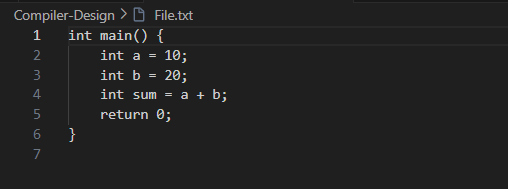
\includegraphics[width=0.8\textwidth]{image/file.png}
    \caption{Sample File}
\end{figure}

\begin{figure}[h]
    \centering
    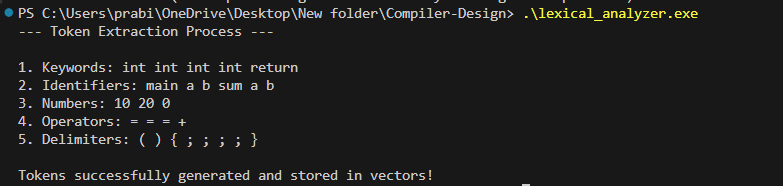
\includegraphics[width=0.8\textwidth]{image/lexical_analyzer.png}
    \caption{Output}
\end{figure}

\section*{Result}
In this way, we were able to read the input file, separate the lexemes and classify them into tokens successfully.

\section*{Code}
The github link to code file: \texttt{https://github.com/vibingprabin/Compiler-Design.git}

\end{document}
